\clearpage
\VerdierPhysicalPageAnchor{0087}%
\VerdierSemanticAnchor{ch1-3-2-2-dual-morphism}
同様に、$\operatorname{tr}_1(C)$ の射

\VerdierSemanticAnchor{ch1-3-2-2-eq3}
\begin{equation}
  \begin{tikzpicture}[>=stealth,baseline=(current bounding box.center)]
    \node (Z)  at (0,1.35) {$0$};
    \node (Y)  at (3.6,1.35) {$Y$};
    \node (X)  at (0,0) {$X$};
    \node (Yp) at (3.6,0) {$Y$};
    \draw[->] (Z) -- (Y);
    \draw[->] (Z) -- (X);
    \draw[->] (Y) -- node[right] {$\operatorname{id}_Y$} (Yp);
    \draw[->] (X) -- node[above] {$f$} (Yp);
  \end{tikzpicture}
  \tag{3.2.2.3}
\end{equation}

\VerdierSemanticAnchor{ch1-3-2-2-cone-entry-p}
に写像錐関手を適用すると、$X\xrightarrow{f}Y$ に関して関手的な
$\operatorname{comp}(C)$ の射 (3.1.2.4)

\VerdierSemanticAnchor{ch1-3-2-2-eq4}
\begin{equation}
  p(f)\colon Y\longrightarrow c(f)
  \tag{3.2.2.4}
\end{equation}
が得られる。

\VerdierSemanticAnchor{ch1-3-2-2-comp-triangle}
したがって、$\operatorname{tr}_1(C)$ の各対象 $X\xrightarrow{f}Y$ に
$\operatorname{comp}(C)$ の三角

\VerdierSemanticAnchor{ch1-3-2-2-eq5}
\begin{equation}
  X\xrightarrow{f}Y\xrightarrow{p(f)}c(f)\xrightarrow{q(f)}X[1]
  \tag{3.2.2.5}
\end{equation}
を対応させることができる。

\VerdierSemanticAnchor{ch1-3-2-2-nonfunctoriality}
この三角は、$\operatorname{tr}_1(C)$ の対象 $X\xrightarrow{f}Y$ に
関手的には依存しないことに注意する。
\VerdierSemanticAnchor{ch1-3-2-2-morphism-d-setup}
実際、
$D=(g,h,a)\colon(X\xrightarrow{f}Y)\longrightarrow
(X'\xrightarrow{f'}Y')$
を $\operatorname{tr}_1(C)$ の射とする。このとき次の図式を得る：

\VerdierSemanticAnchor{ch1-3-2-2-eq6}
\begin{equation}
  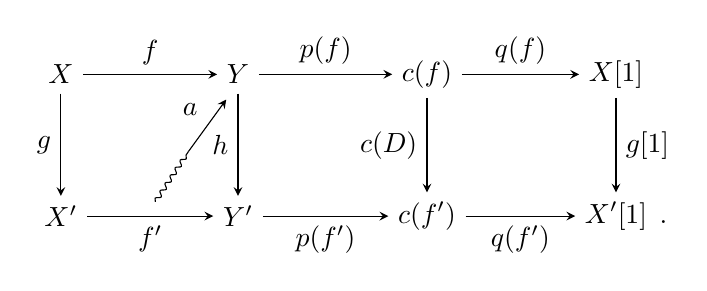
\begin{tikzpicture}[>=stealth,baseline=(current bounding box.center)]
    \node (X)   at (0,1.8) {$X$};
    \node (Y)   at (2.25,1.8) {$Y$};
    \node (C)   at (4.65,1.8) {$c(f)$};
    \node (Xs)  at (7.05,1.8) {$X[1]$};
    \node (Xp)  at (0,0) {$X'$};
    \node (Yp)  at (2.25,0) {$Y'$};
    \node (Cp)  at (4.65,0) {$c(f')$};
    \node (Xps) at (7.05,0) {$X'[1]$};
    \node[anchor=base west,inner sep=0pt,xshift=.08em] at (Xps.base east) {$.$};
    \draw[->] (X) -- node[above] {$f$} (Y);
    \draw[->] (Y) -- node[above] {$p(f)$} (C);
    \draw[->] (C) -- node[above] {$q(f)$} (Xs);
    \draw[->] (Xp) -- node[below] {$f'$} (Yp);
    \draw[->] (Yp) -- node[below] {$p(f')$} (Cp);
    \draw[->] (Cp) -- node[below] {$q(f')$} (Xps);
    \draw[->] (X) -- node[left] {$g$} (Xp);
    \draw[->] (Y) -- node[left] {$h$} (Yp);
    \draw[->] (C) -- node[left] {$c(D)$} (Cp);
    \draw[->] (Xs) -- node[right] {$g[1]$} (Xps);
    \draw[decorate,decoration={snake,amplitude=0.8pt,segment length=3.3pt}]
      (1.20,0.18) -- (1.62,0.82);
    \draw[->] (1.62,0.82) -- node[above left] {$a$} (2.10,1.48);
  \end{tikzpicture}
  \tag{3.2.2.6}
\end{equation}

\VerdierSemanticAnchor{ch1-3-2-2-square-commutativity}
射 $p(f)$ と $q(f)$ は $f$ に関して関手的であるから、この図式の後ろ二つの
正方形は可換であるが、最初の正方形はホモトピーを除いてのみ可換である。
\VerdierSemanticAnchor{ch1-3-2-2-quotient-triangle}
ホモトピーで商をとると、$\operatorname{Tr}_1(C)$ の各対象
$X\xrightarrow{f}Y$ に $K(C)$ の三角

\VerdierSemanticAnchor{ch1-3-2-2-eq7}
\begin{equation}
  X\xrightarrow{\dot f}Y\xrightarrow{\dot p(f)}c(f)
  \xrightarrow{\dot q(f)}X[1]
  \tag{3.2.2.7}
\end{equation}
\VerdierSemanticAnchor{ch1-3-2-2-homotopy-class-notation}
を関手的に対応させることができる。（$\dot f$、$\dot p(f)$、
$\dot q(f)$ は、それぞれ射 $f$、$p(f)$、$q(f)$ のホモトピー類を表す。）
\VerdierSemanticAnchor{ch1-3-2-2-triangle-functor}
こうして、圏 $\operatorname{Tr}_1(C)$ から $K(C)$ における三角の圏への
関手を得る。
